\documentclass[12pt, a4paper]{article}

\usepackage{amsmath}
\usepackage{bm}
\usepackage{array}
\usepackage{amsmath}
\usepackage[portuguese]{babel}
\usepackage{chngpage}
\usepackage{float}
\usepackage[a4paper, margin=2cm]{geometry}
\usepackage{graphicx}
\usepackage{hyperref}
\usepackage{listings}
\usepackage{setspace}
\usepackage{xcolor}

\lstdefinestyle{codestyle}{
    commentstyle=\color{teal},
    keywordstyle=\color{blue},
    numberstyle=\ttfamily\color{gray},
    stringstyle=\color{red},
    basicstyle=\ttfamily\footnotesize,
    breakatwhitespace=false,
    breaklines=false,
    keepspaces=true,
    numbers=none,
    showspaces=false,
    showstringspaces=false,
    showtabs=false,
    tabsize=4
}
\lstset{style=codestyle}

\title{\Huge \textbf{Computação Gráfica \\ \Large Trabalho Prático -- Fase IV}}
\date{18 de maio de 2025}
\author{Grupo 3}

\begin{document}

\begin{center}
    
\includegraphics[width=0.25\textwidth]{res/cover/EE-C.eps}
\end{center}

\chardef\_=`_
\onehalfspacing
\setlength{\parskip}{\baselineskip}
\setlength{\parindent}{0pt}
\def\arraystretch{1.5}

{\let\newpage\relax\maketitle}
\maketitle
\thispagestyle{empty}

\vspace*{\fill}

\begin{adjustwidth}{-2cm}{-2cm} % These values only need to be large enough to center the table
    \begin{center}
        \begin{tabular}{>{\centering}p{0.25\textwidth}
                        >{\centering}p{0.25\textwidth}
                        >{\centering}p{0.25\textwidth}
                        >{\centering\arraybackslash}p{0.25\textwidth}}
            
\includegraphics[width=3.5cm]{res/cover/A104437.png} &
            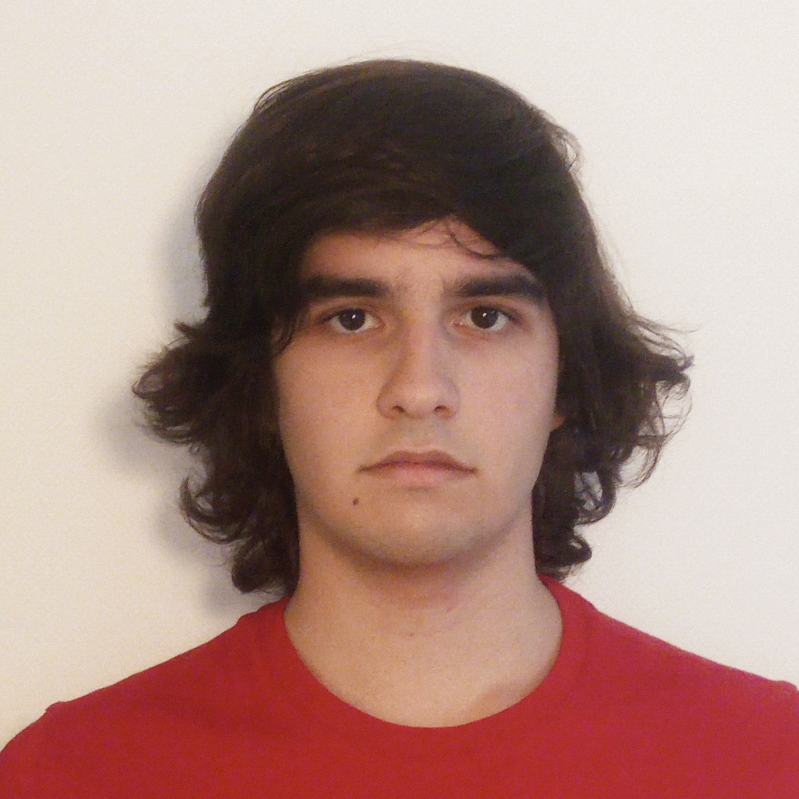
\includegraphics[width=3.5cm]{res/cover/A104348.png} &
            
\includegraphics[width=3.5cm]{res/cover/A90817.png} &
            
\includegraphics[width=3.5cm]{res/cover/A104179.png} \\

            Ana Oliveira & Humberto Gomes & Mariana Cristino & Sara Lopes \\
            A104437      & A104348        & A90817           & A104179
        \end{tabular}
    \end{center}
\end{adjustwidth}

\pagebreak

\begin{abstract}
    \noindent
    {\color{red} TODO - Humberto}
\end{abstract}

\section{\emph{Generator}}

\subsection{Formato \texttt{.3d}}

O formato \texttt{.3d} exportado pelo \texttt{generator} e utilizado pela \texttt{engine} é o
Wavefront OBJ \cite{wavefront-obj}. Apenas uma pequena fração das funcionalidades deste formato
são suportadas e, nesta fase, foram necessárias adições aos mecanismos de escrita e leitura de
ficheiros Wavefront OBJ para suportar coordenadas de textura e normais. Este formato é textual, onde
cada linha pode ser um comentário, uma posição, uma coordenada de textura, uma normal, ou uma face
triangular, como mostra o exemplo abaixo, na ordem apresentada:

\begin{lstlisting}

# Comment
v 0.5 0.5 1
vt 0.3 0.3
vn 0 1 0
f 1/2/3 4/5/6 7/8/9
\end{lstlisting}

Quando uma linha começa com \texttt{v}, \texttt{vt} ou \texttt{vn}, devem seguir-se as coordenadas
de uma posição, de uma textura, ou de um vetor normal, respetivamente. Quando uma linha começa com
\texttt{f}, deve seguir-se uma face triangular, ou seja três pontos. O \texttt{generator} e a
\texttt{engine} suportam dois tipos de ponto:

\begin{itemize}
    \item Apenas um número, um índice de uma posição, ou seja, um elemento do tipo \texttt{v}
        (começando a contar em 1);
    \item Da forma \texttt{v/t/n}, onde estão presentes três índices, um para uma posição, um para
        uma coordenada de textura, e outro para um vetor normal.
\end{itemize}

Como o \emph{parser} de ficheiros Wavefront OBJ foi reimplementado na fase anterior com base em
expressões regulares, foi trivial adicionar o suporte para coordenadas de textura e vetores normais.

\subsection{Plano Horizontal}

{\color{red} TODO - Humberto}

\subsection{Cubo}

{\color{red} TODO - Humberto}

\subsection{Esfera}

{\color{red} TODO - Mariana}

\subsection{Cone}

{\color{red} TODO - Ana}

\subsection{Cilindro}

{\color{red} TODO - Mariana}

\subsection{\emph{Torus}}

{\color{red} TODO - Sara}

\subsection{Outras Figuras}

Para as restantes figuras, devido à sua complexidade e ao pouco tempo disponível para a conclusão
desta fase do trabalho prático, não foram adicionadas nem coordenadas de textura nem normais. No
entanto, a \texttt{engine} ainda é capaz de importar estes modelos e de os desenhar com iluminação,
graças a um algoritmo de geração automática de normais implementado e descrito posteriormente neste
relatório.

\subsection{Sistema Solar}

{\color{red} TODO - Ana}

\section{\emph{Engine}}

\subsection{Geração Automática de Normais}

A \texttt{engine} é capaz de carregar modelos que não tenham informação sobre coordenadas de
texturas ou normais. Caso não haja informação sobre as coordenadas de textura de um modelo, é
possível desenhá-lo a uma cor sólida, mas é necessário que se tenha informação sobre as suas normais
para o iluminar corretamente. Como esta nem sempre está presente, foi implementado um algoritmo para
gerar normais de modelos automaticamente.

Este algoritmo considera o modelo inteiro como um único \emph{smoothing group}, e calcula a normal
de cada vértice como a média das normais dos triângulos a que este pertence, pesada pela área dos
triângulos. Logo, é necessário, em primeiro lugar, uma forma de calcular a normal de um triângulo.
Para um triângulo $[ABC]$, esta pode ser calculada do seguinte modo:

$$
\hat{n}_{[ABC]} = \frac{
    \overrightarrow{AB} \times \overrightarrow{AC}
}{
    \lVert \overrightarrow{AB} \times \overrightarrow{AC} \rVert
}
$$

Depois, a área de cada triângulo, $A$, pode ser calculada pela fórmula de Heron:

$$
S = \frac{
    \lVert \overrightarrow{AB} \rVert +
    \lVert \overrightarrow{AC} \rVert +
    \lVert \overrightarrow{BC} \rVert
}{
    2
}
$$

$$
A = \sqrt{
    S
    \left ( S - \lVert \overrightarrow{AB} \rVert \right )
    \left ( S - \lVert \overrightarrow{AC} \rVert \right )
    \left ( S - \lVert \overrightarrow{BC} \rVert \right )
}
$$

Logo, sendo $F$ o conjunto de faces triangulares nas quais um ponto está presente, o vetor normal
desse ponto é dado por:

$$
\hat{n} = \frac{
    \sum_{f \in F} {A_f \, \hat{n}_f}
}{
    \lVert \sum_{f \in F} {A_f \, \hat{n}_f} \rVert
}
$$

Em termos de implementação deste algoritmo, um dicionário é utilizado para armazenar associações
entre posições de pontos e pares normal-área. Iteram-se por todas as faces do modelo e, para
cada face, calcula-se a sua normal e a sua área. Depois, para cada ponto nessa face, adicionam-se
aos valores armazenados de normal e de área $A \, \hat{n}$ e $A$ respetivamente. Após iterar por
todas as faces, itera-se por todas as posições no dicionário, e define-se a normal de cada ponto
como o quociente entre a normal armazenada e a área total. Logicamente, este vetor deve ser
normalizado antes de adicionado ao modelo.

\subsection{Adição ao \emph{Schema} XML}

{\color{red} TODO - Mariana}

\subsection{Texturas e Normais}

{\color{red} TODO - Humberto}

\subsection{\emph{Object Picking}}

{\color{red} TODO - Sara}

\section{Resultados Obtidos}

{\color{red} TODO - cada faz as suas prints, sem borda de janela, no tamanho especificado pela cena,
com a UI escondida (U), Humberto escreve}

\section{Conclusão}

{\color{red} TODO - Humberto}

\begingroup
\section{Bibliografia}
\renewcommand{\section}[2]{}

\begin{thebibliography}{9}
    \bibitem{wavefront-obj}
        "Wavefront OBJ File Format Summary."{} FileFormat.Info. Accessed: May 14, 2025. [Online.]
        Available: \url{https://www.fileformat.info/format/wavefrontobj/egff.htm}
\end{thebibliography}
\endgroup

\end{document}
